% !TEX program = xelatex
% 공통수학2 · Ⅰ. 도형의 방정식 · 02 직선의 위치 관계 · 1/2차시
% 학생용 활동지 (답안 없음)

\documentclass[11pt,a4paper]{article}

\usepackage{kotex}
\usepackage{iftex}
\ifPDFTeX\else
  \setmainhangulfont{Noto Serif CJK KR}
  \setsanshangulfont{Noto Sans CJK KR}
\fi

\usepackage[margin=2.1cm]{geometry}
\usepackage{parskip}
\usepackage{enumitem}
\usepackage{array}
\usepackage{tabularx}
\usepackage{xcolor}
\usepackage{amssymb}
\usepackage{tikz}
\usepackage[most]{tcolorbox}
\usepackage{fancyhdr}
\usepackage{titlesec}

\definecolor{goldc}{HTML}{B07C22}
\definecolor{goldstrong}{HTML}{8A5F16}
\definecolor{indigoc}{HTML}{2B3B57}
\definecolor{indigosoft}{HTML}{6E82A6}
\definecolor{linec}{HTML}{D6DACB}
\definecolor{surface2}{HTML}{E4E8DC}
\definecolor{writeline}{HTML}{C7CCBA}
\definecolor{inksoft}{HTML}{52604F}

\titleformat{\section}
  {\normalfont\sffamily\bfseries\large\color{indigoc}}
  {\thesection}{0.6em}{}
\titlespacing{\section}{0pt}{14pt}{6pt}

\newtcolorbox{goalbox}{enhanced, breakable, colback=white, colframe=goldc, boxrule=0.5pt, leftrule=3pt, arc=2pt, left=10pt, right=10pt, top=8pt, bottom=8pt}
\newtcolorbox{sheetbox}{enhanced, breakable, colback=white, colframe=linec, boxrule=0.6pt, arc=3pt, left=11pt, right=11pt, top=9pt, bottom=9pt}

\newcommand{\writespace}[1]{%
  \par\nobreak\vspace{3pt}
  \foreach \n in {1,...,#1} {%
    \noindent\textcolor{writeline}{\rule{\linewidth}{0.4pt}}\par\vspace{0.62cm}%
  }
}
\newcommand{\fillblank}[1]{\makebox[#1]{\hrulefill}}

\pagestyle{fancy}
\fancyhf{}
\renewcommand{\headrulewidth}{0pt}
\fancyfoot[L]{\footnotesize\color{inksoft} 공통수학2 · 2026학년도 2학기 · 지평선고등학교}
\fancyfoot[R]{\footnotesize\color{inksoft} 다음 시간 --- 02 직선의 위치 관계(2) 수직 조건}

\begin{document}

\noindent
\begin{minipage}[b]{0.62\linewidth}
  {\sffamily\footnotesize\color{indigosoft} 공통수학2 · Ⅰ. 도형의 방정식}\\[2pt]
  {\sffamily\bfseries\Large 02 직선의 위치 관계 \textperiodcentered\ 4차시}
\end{minipage}\hfill
\begin{minipage}[b]{0.36\linewidth}
  \raggedleft\small\color{inksoft}
  반\ \fillblank{1.6cm} \quad 번호\ \fillblank{1.6cm}\\[4pt]
  이름\ \fillblank{3.6cm}
\end{minipage}

\vspace{4pt}
\noindent{\color{goldc}\rule{\linewidth}{2.2pt}}
\vspace{10pt}

\begin{goalbox}
\textbf{오늘의 목표}\\
두 직선이 평행하기 위한 조건을 알고, 한 점을 지나고 주어진 직선에 평행한 직선의 방정식을 구할 수 있다.
\vspace{4pt}

\small\color{inksoft}
$\square$ 자신 있음 \quad $\square$ 조금 헷갈림 \quad $\square$ 처음 봄 \hfill (수업 전 나의 상태에 표시)
\end{goalbox}

\section{생각 열기 --- 에스컬레이터의 기울기}

\begin{sheetbox}
어느 건물의 에스컬레이터를 좌표평면 위에 나타냈다. 직선 $l$은 두 점 $(0,3)$과 $(4,5)$를, 직선 $m$은 두 점 $(0,1)$과 $(2,2)$를 지난다.

\begin{center}
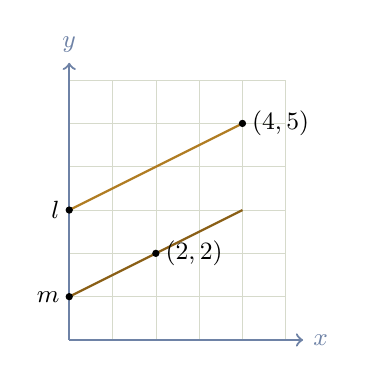
\begin{tikzpicture}[scale=0.55]
  \draw[step=1cm, linec, very thin] (0,0) grid (5,6);
  \draw[->, thick, indigosoft] (0,0) -- (5.4,0) node[right, font=\small]{$x$};
  \draw[->, thick, indigosoft] (0,0) -- (0,6.4) node[above, font=\small]{$y$};
  \draw[thick, goldc] (0,3) -- (4,5);
  \draw[thick, goldstrong] (0,1) -- (4,3);
  \node[left, font=\small] at (0,3) {$l$};
  \node[right, font=\small] at (4,5) {$(4,5)$};
  \node[left, font=\small] at (0,1) {$m$};
  \node[right, font=\small] at (2,2) {$(2,2)$};
  \filldraw (0,3) circle (2pt);
  \filldraw (4,5) circle (2pt);
  \filldraw (0,1) circle (2pt);
  \filldraw (2,2) circle (2pt);
\end{tikzpicture}
\end{center}

\begin{enumerate}[leftmargin=1.4em, itemsep=2pt]
  \item 두 직선 $l$과 $m$의 기울기를 각각 구해 보자.
  \item 두 직선 $l$과 $m$이 서로 평행한지 말해 보자.
\end{enumerate}
\writespace{3}
\end{sheetbox}

\section{개념 정리 --- 두 직선의 평행 조건}

\begin{sheetbox}
두 직선 $y=mx+n$과 $y=m'x+n'$에 대하여

\begin{enumerate}[leftmargin=1.6em, itemsep=4pt]
  \item 두 직선이 서로 평행하면, $m=\fillblank{1.6cm}$이고 $n\ \fillblank{1.6cm}\ n'$.
  \item $m=m'$이고 $n\neq n'$이면, 두 직선은 \fillblank{3.6cm}.
\end{enumerate}

\vspace{4pt}
\textbf{주의} --- $m=m'$이고 $n=n'$이면, 두 직선은 \fillblank{3.6cm}.
\end{sheetbox}

\section{연습 문제}

\begin{sheetbox}
\textbf{1.} 다음 직선의 방정식을 구하시오.\\
\hspace*{1.6em}⑴ 점 $(3,-4)$를 지나고 기울기가 $2$인 직선 \qquad ⑵ 점 $(-1,5)$를 지나고 $x$축에 평행한 직선
\writespace{2}

\vspace{8pt}
\textbf{2.} 점 $(-2,-4)$를 지나고 다음 직선에 평행한 직선의 방정식을 구하시오.\\
\hspace*{1.6em}⑴ $y=-2x-1$ \qquad ⑵ $3x-2y+5=0$
\writespace{3}

\vspace{8pt}
\textbf{3.} 점 $(2,3)$을 지나고 직선 $2x-y+1=0$에 평행한 직선의 방정식을 구하시오.
\writespace{2}
\end{sheetbox}

\section{사고의 가시화 --- See · Think · Wonder}

\noindent{\footnotesize\color{inksoft} 오늘 배운 `평행 조건'을 떠올리며 아래 세 칸을 채워 보자.}\\[6pt]
\begin{tabularx}{\linewidth}{@{}XXX@{}}
\textbf{\footnotesize\color{indigoc} See --- 무엇을 보았나?} &
\textbf{\footnotesize\color{indigoc} Think --- 무엇을 생각했나?} &
\textbf{\footnotesize\color{indigoc} Wonder --- 무엇이 궁금한가?} \\[4pt]
\end{tabularx}
\noindent
\begin{minipage}[t]{0.32\linewidth}\writespace{3}\end{minipage}\hfill
\begin{minipage}[t]{0.32\linewidth}\writespace{3}\end{minipage}\hfill
\begin{minipage}[t]{0.32\linewidth}\writespace{3}\end{minipage}

\section{마무리 성찰}

\begin{sheetbox}
\begin{minipage}[t]{0.48\linewidth}
{\footnotesize\color{inksoft} 오늘 배운 것을 한 문장으로}
\writespace{2}
\end{minipage}\hfill
\begin{minipage}[t]{0.48\linewidth}
{\footnotesize\color{inksoft} 감사 일기 / 유념 한 줄}
\writespace{2}
\end{minipage}
\end{sheetbox}

\end{document}
